The software the system will need will take in a row vector of position, orientation, path type, and end effector function information for all points to be traveled through and run the manipulator through the desired points following the specified paths requested. To do this, the user will first be asked what the number of points being input will be so that a few data structures can be preallocated. The user will then be asked if the manipulator will be writing or doing pick and place, and store the response. If the user is doing pick and place, the user will be asked for the full point data consisting of the x, y, and z location in millimeters, the phi, theta, and psi angles in degrees, the path type, and the end effector function. If the user is doing writing, only the x, y, and z locations will be requested. The orientation of the point will be defaulted in the “down” orientation since the marker will be held vertically, the path type will be set to cartesian straight line, and the end effector function will be set to stay unchanged. When all the desired points have been input, the software will then create intermediate points every centimeter between points whose paths are specified as cartesian straight line and store the new path points in a different data structure. After the path has been created, each point will be run through inverse kinematics to get the required joint angles to achieve the position and will be stored as the motor data for each point. If the user is writing with the manipulator, the user will be prompted to press a key to close the end effector to grab the marker. The user will then be prompted to press a key to begin, at which point the software will send the motor data to each servo for the first point that the system is trying to reach, wait till the servos are in the desired position, run the end effector function if there is one, and then repeat the process with the next set of motor data until all the points have been traveled through. When the last point has been reached, the program will prompt the user to input the number of desired points and wait for the input to start the process over again.
\captionsetup[sub]{
    labelformat=r-parens}
The software the system uses takes in a row vector of position, orientation, path type, and end effector function information for all points to be traveled through and runs the manipulator through the desired points following the specified paths requested. The general overview of the code is shown in \emph{Figure \ref{fig:soverall}}.

\begin{figure}[htp]
  \center
  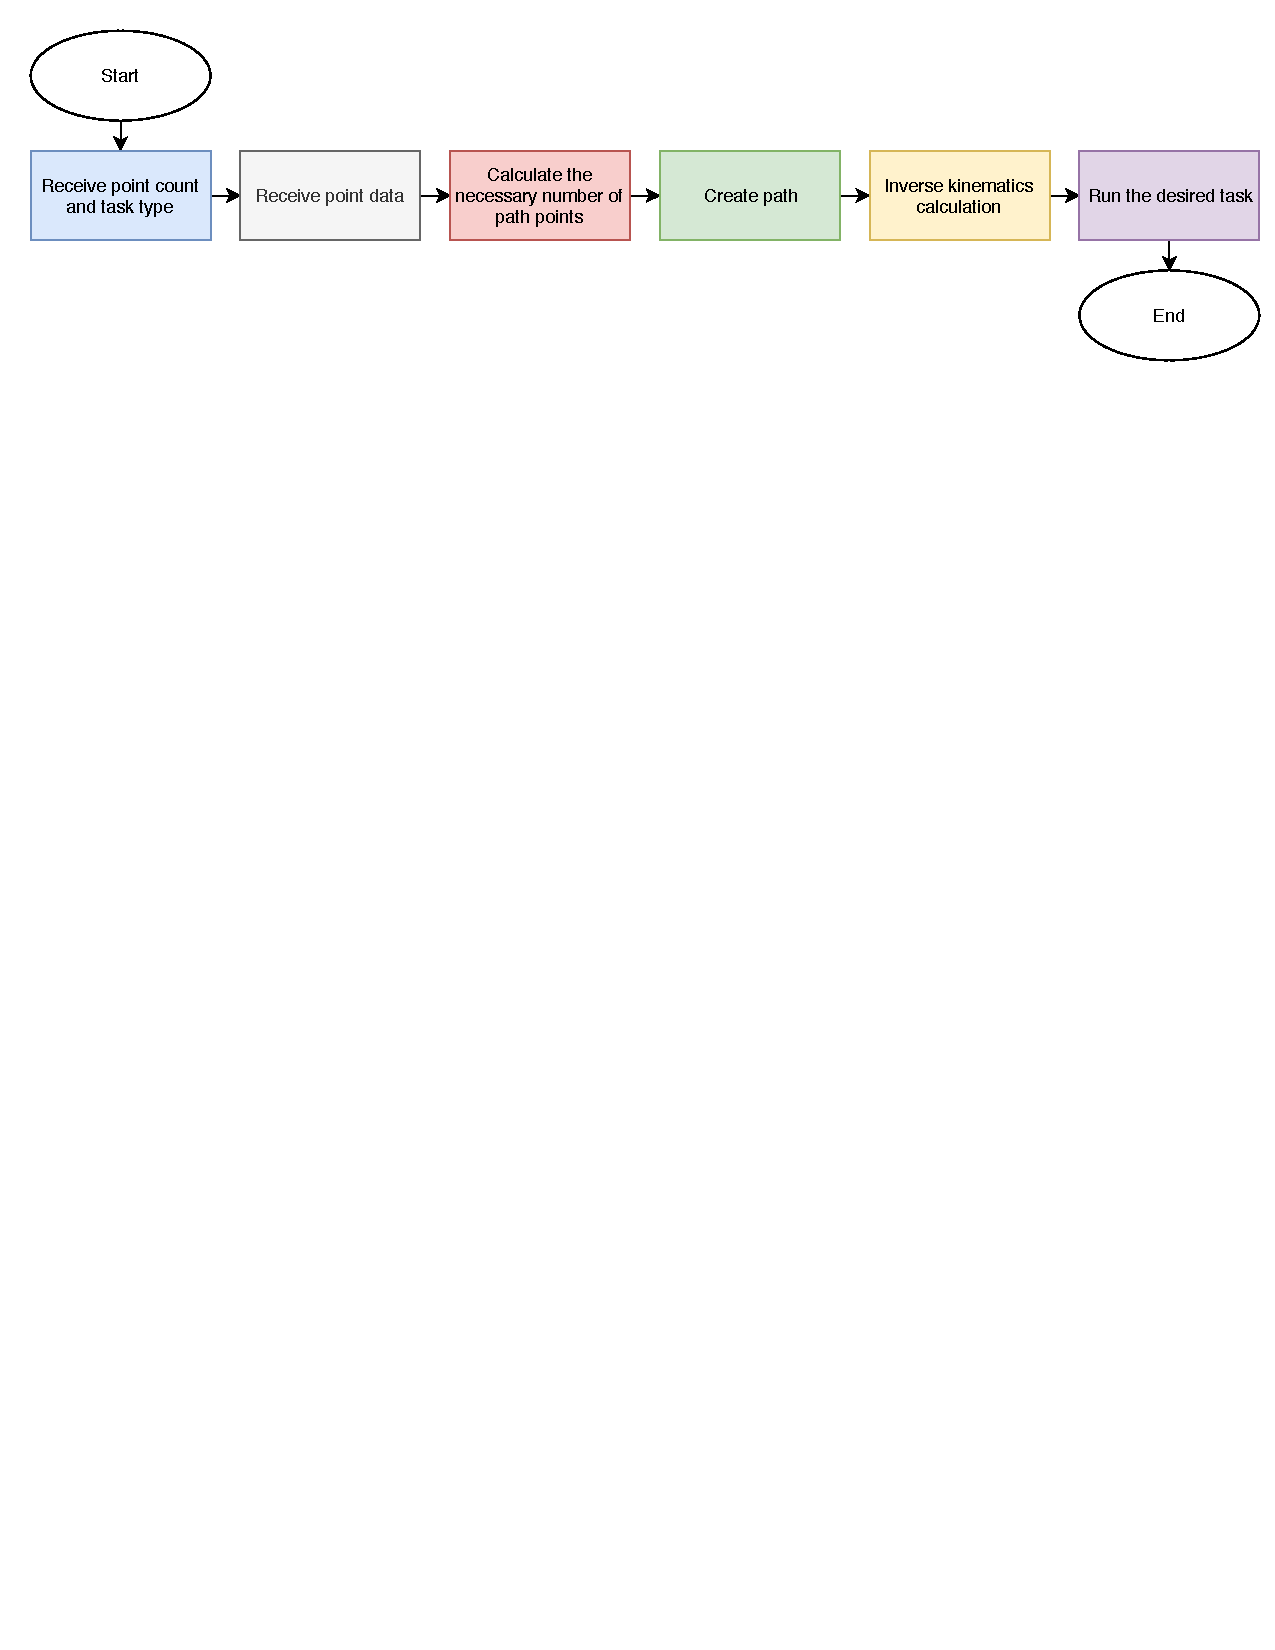
\includegraphics[width=\textwidth]{soverall}
  \caption{Software Flowchart}
  \label{fig:soverall}
\end{figure}

\emph{Figure \ref{fig:soverall}} shows that the software for the manipulator is broken up into six subsections, two sections that receive data, three that do calculations, and one that runs the specified task.

The first subsection of the software works to receive the number of points the user is inputting as well as the general task the user is completing, shown in \emph{Figure \ref{fig:sf1}}. \\

\begin{figure}[htp] \ContinuedFloat
  \begin{subfigure}[c]{\textwidth}
  \center
  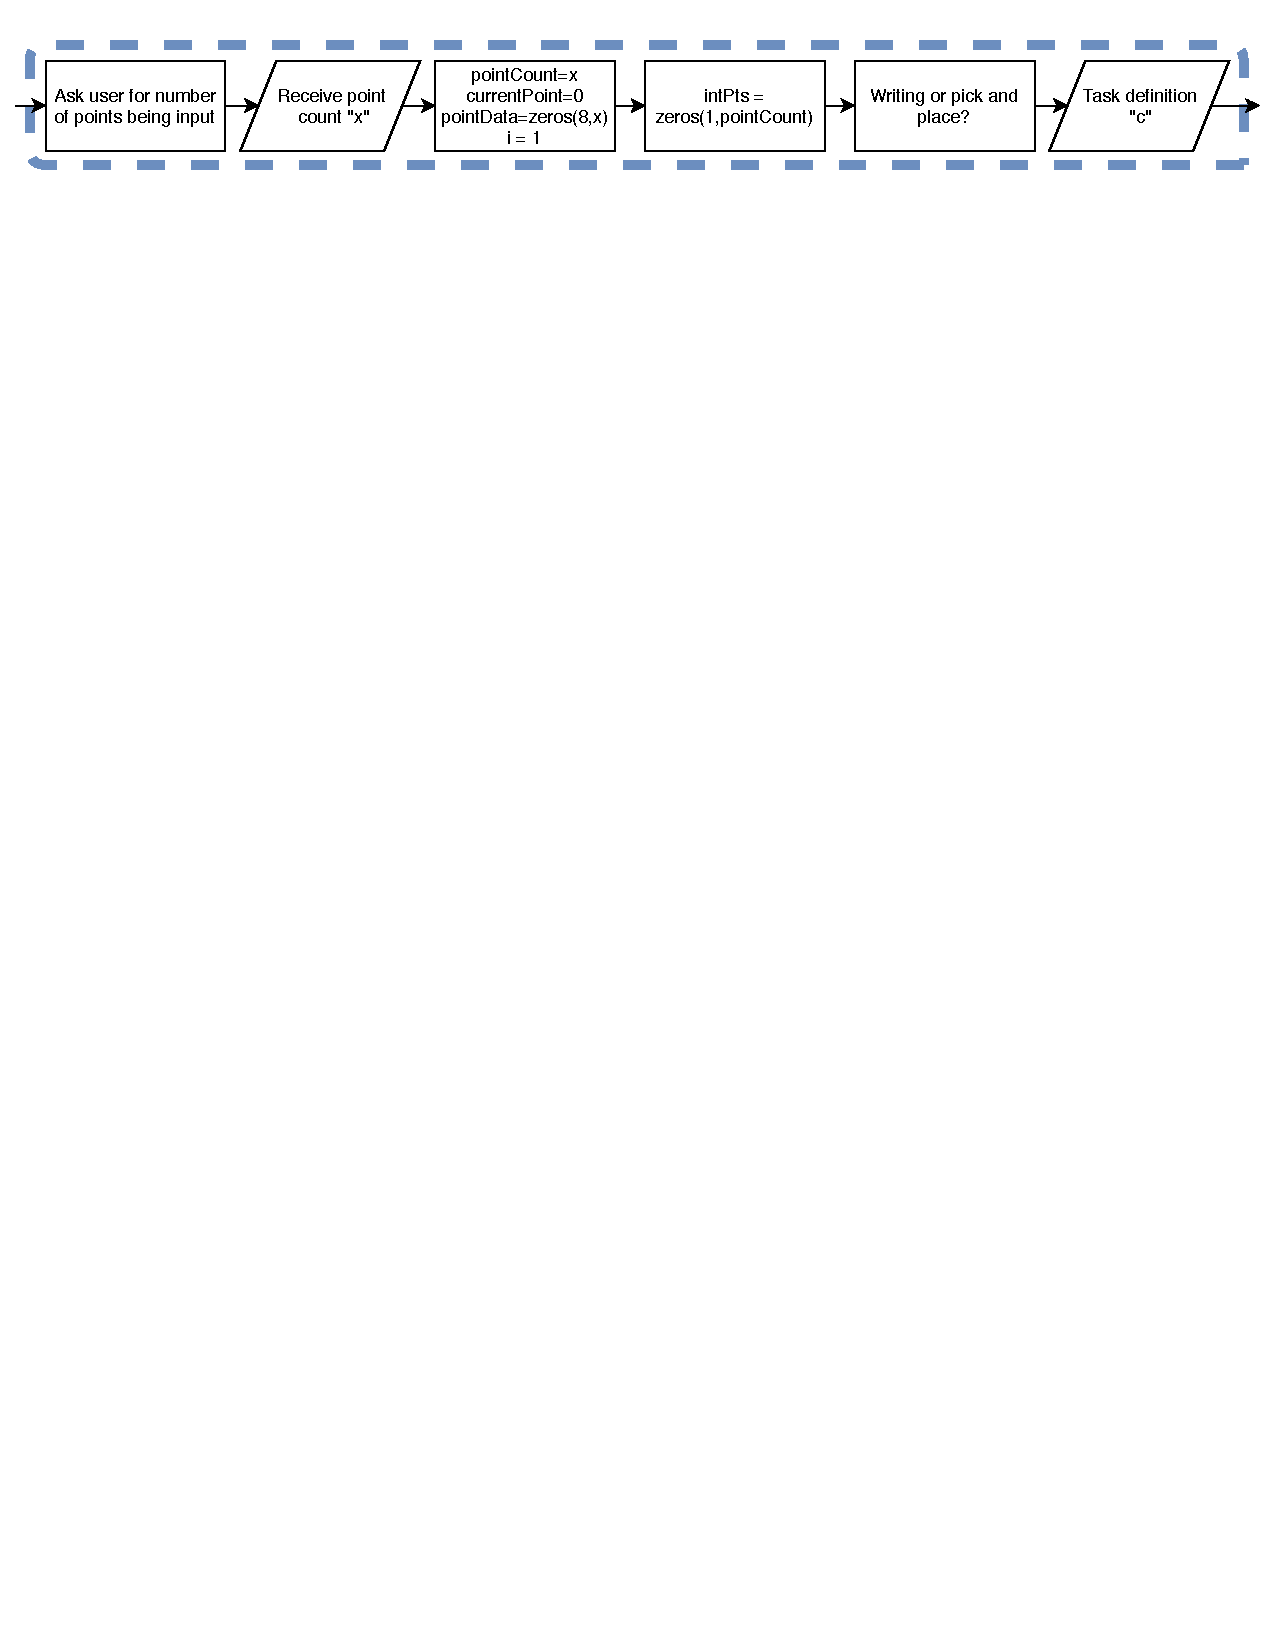
\includegraphics[width=\textwidth]{sf1}
  \caption{Software Flowchart Subsection 1}
  \label{fig:sf1}
  \end{subfigure}
\end{figure}

\emph{Figure \ref{fig:sf1}} specifies that the software prompts the user for the number of points that the manipulator will travel through and stores the input as a variable, in this case ‘x’. The ‘x’ variable is only used to help preallocate data vectors so that the size of the vector does not change with each input. The software also receives the task specification as either a 0 for cartesian straight line pathing or a 1 for a straight line in the joint space and stores this value in the variable ‘c’.

The second general block in the software flowchart works to receive and store the necessary data for the points the user is inputting depending on the path type as seen in \emph{Figure \ref{fig:sf2}}.
\begin{figure}[htp] \ContinuedFloat
  \begin{subfigure}[c]{\textwidth}
  \center
  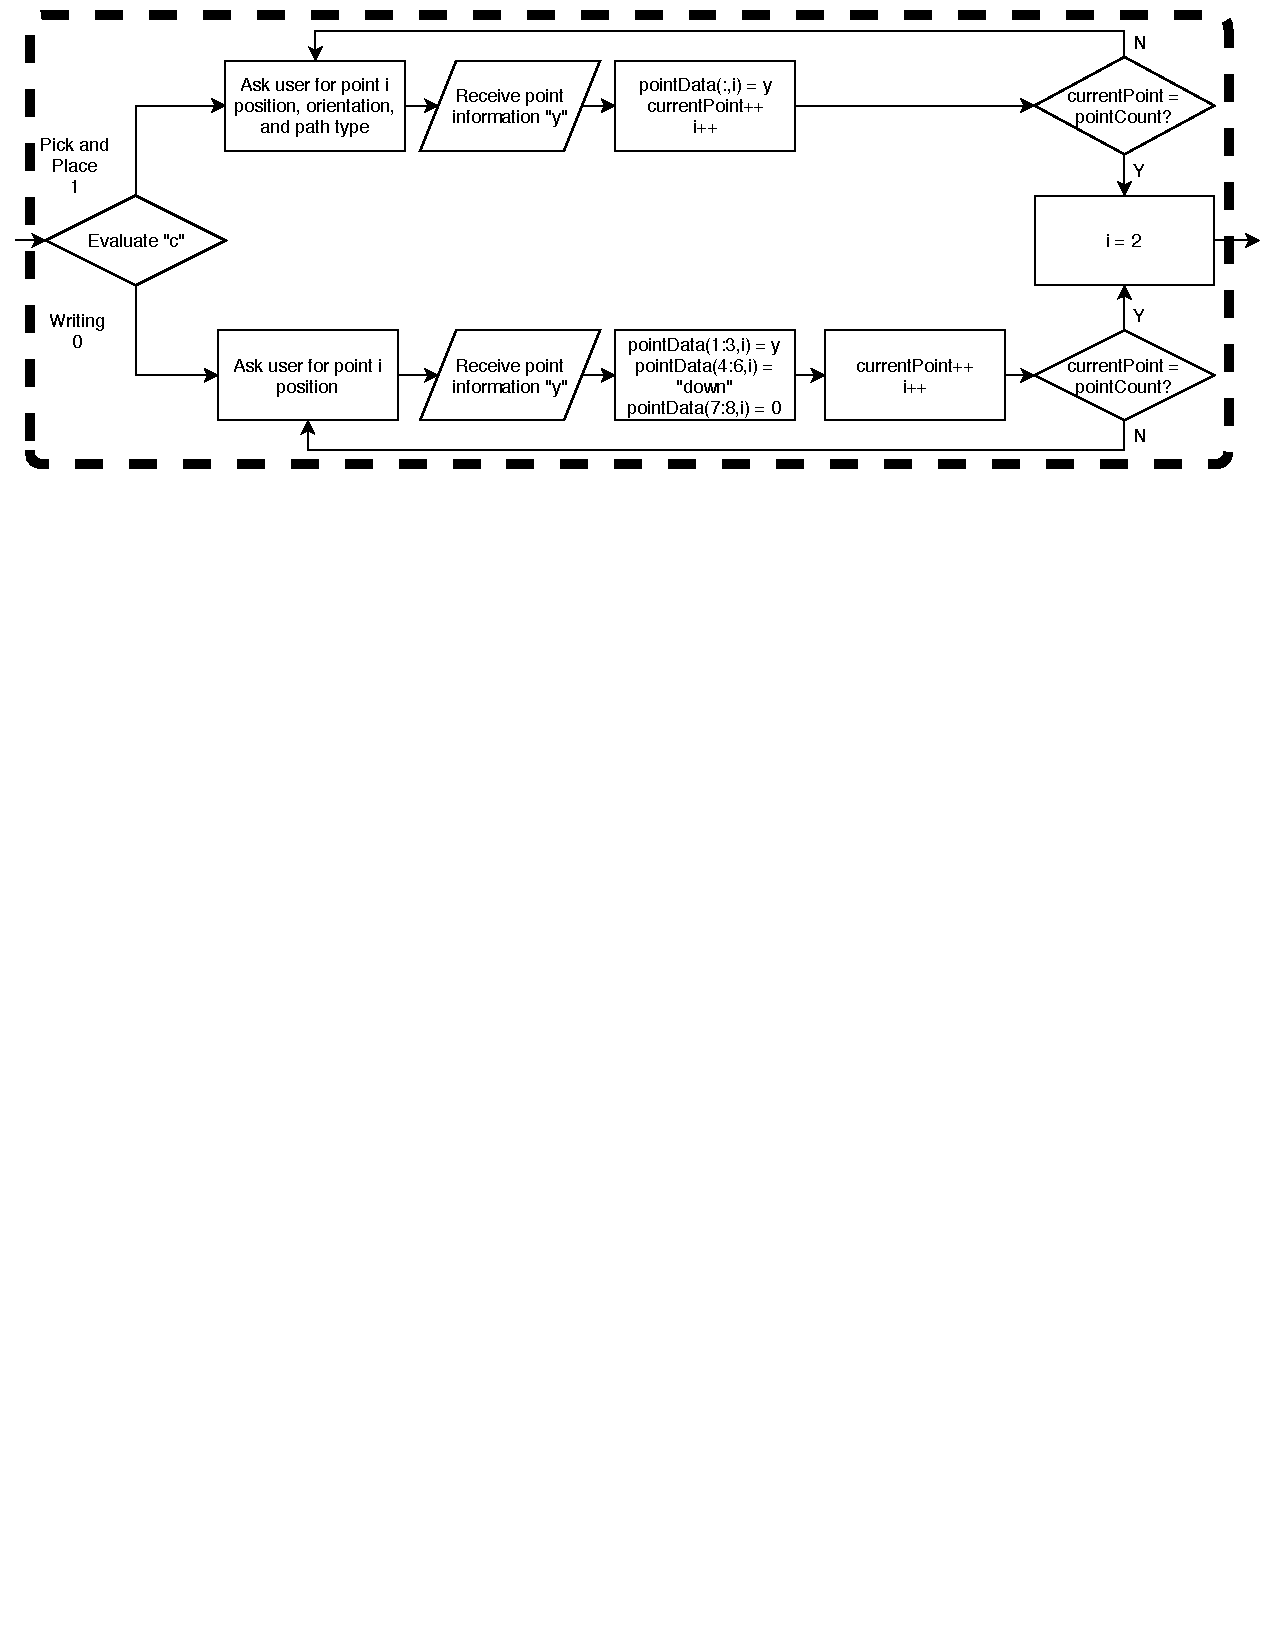
\includegraphics[width=\textwidth]{sf2}
  \caption{Software Flowchart Subsection 2}
  \label{fig:sf2}
\end{subfigure}
\end{figure}

\emph{Figure \ref{fig:sf2}} shows that the path type variable ‘c’ is used to determine what information is necessary to collect. If the user is doing a writing task, the software only collects the x, y, and z distances for the point and assumes that the end effector orientation will be facing down so that the marker is vertical. If the user is doing pick and place, the software prompts the user for the x, y, z, phi, theta, psi, path type, and end effector data. The software loops until all the points have been input.

The next block in the software flowchart calculates the total points necessary to complete the task. The overview for this section can be seen in \emph{Figure \ref{fig:sf3}}.

\begin{figure}[htp]\ContinuedFloat
  \begin{subfigure}[c]{\textwidth}
  \center
  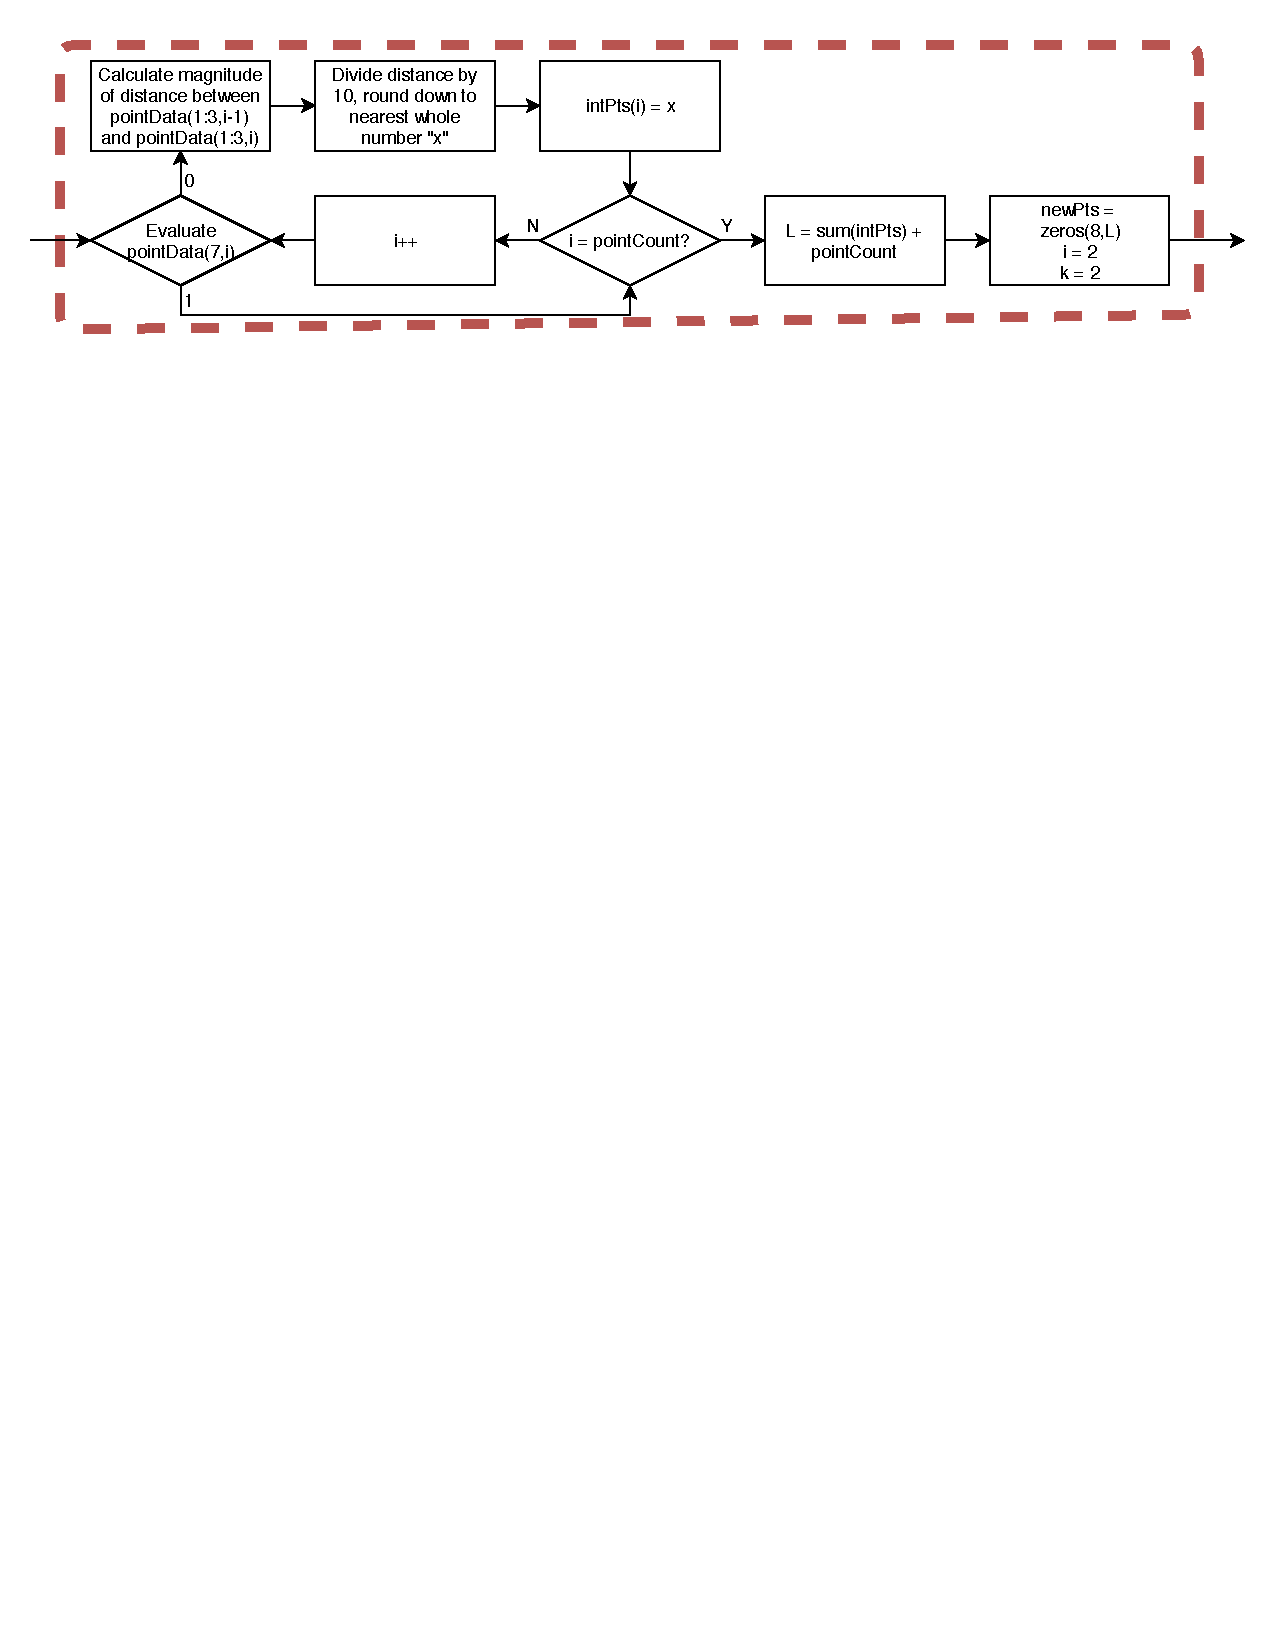
\includegraphics[width=\textwidth]{sf3}
  \caption{Software Flowchart Subsection 3}
  \label{fig:sf3}
  \end{subfigure}
\end{figure}

As seen in \emph{Figure \ref{fig:sf3}}, the section of software calculates the distance between the current point and the previous point if the path type is cartesian straight line and divides the distance by ten to find the number of centimeters between the two points. This value is stored as the necessary number of intermediate points, and the software will loop through until every point has been checked. The section of code also stores the total number of points that will be used as the variable level for later use.

The fourth code block in the flowchart creates and stores the necessary intermediate points along the desired path, shown in \emph{Figure \ref{fig:sf4}}.

\begin{figure}[htp] \ContinuedFloat
  \begin{subfigure}[c]{\textwidth}
  \center
  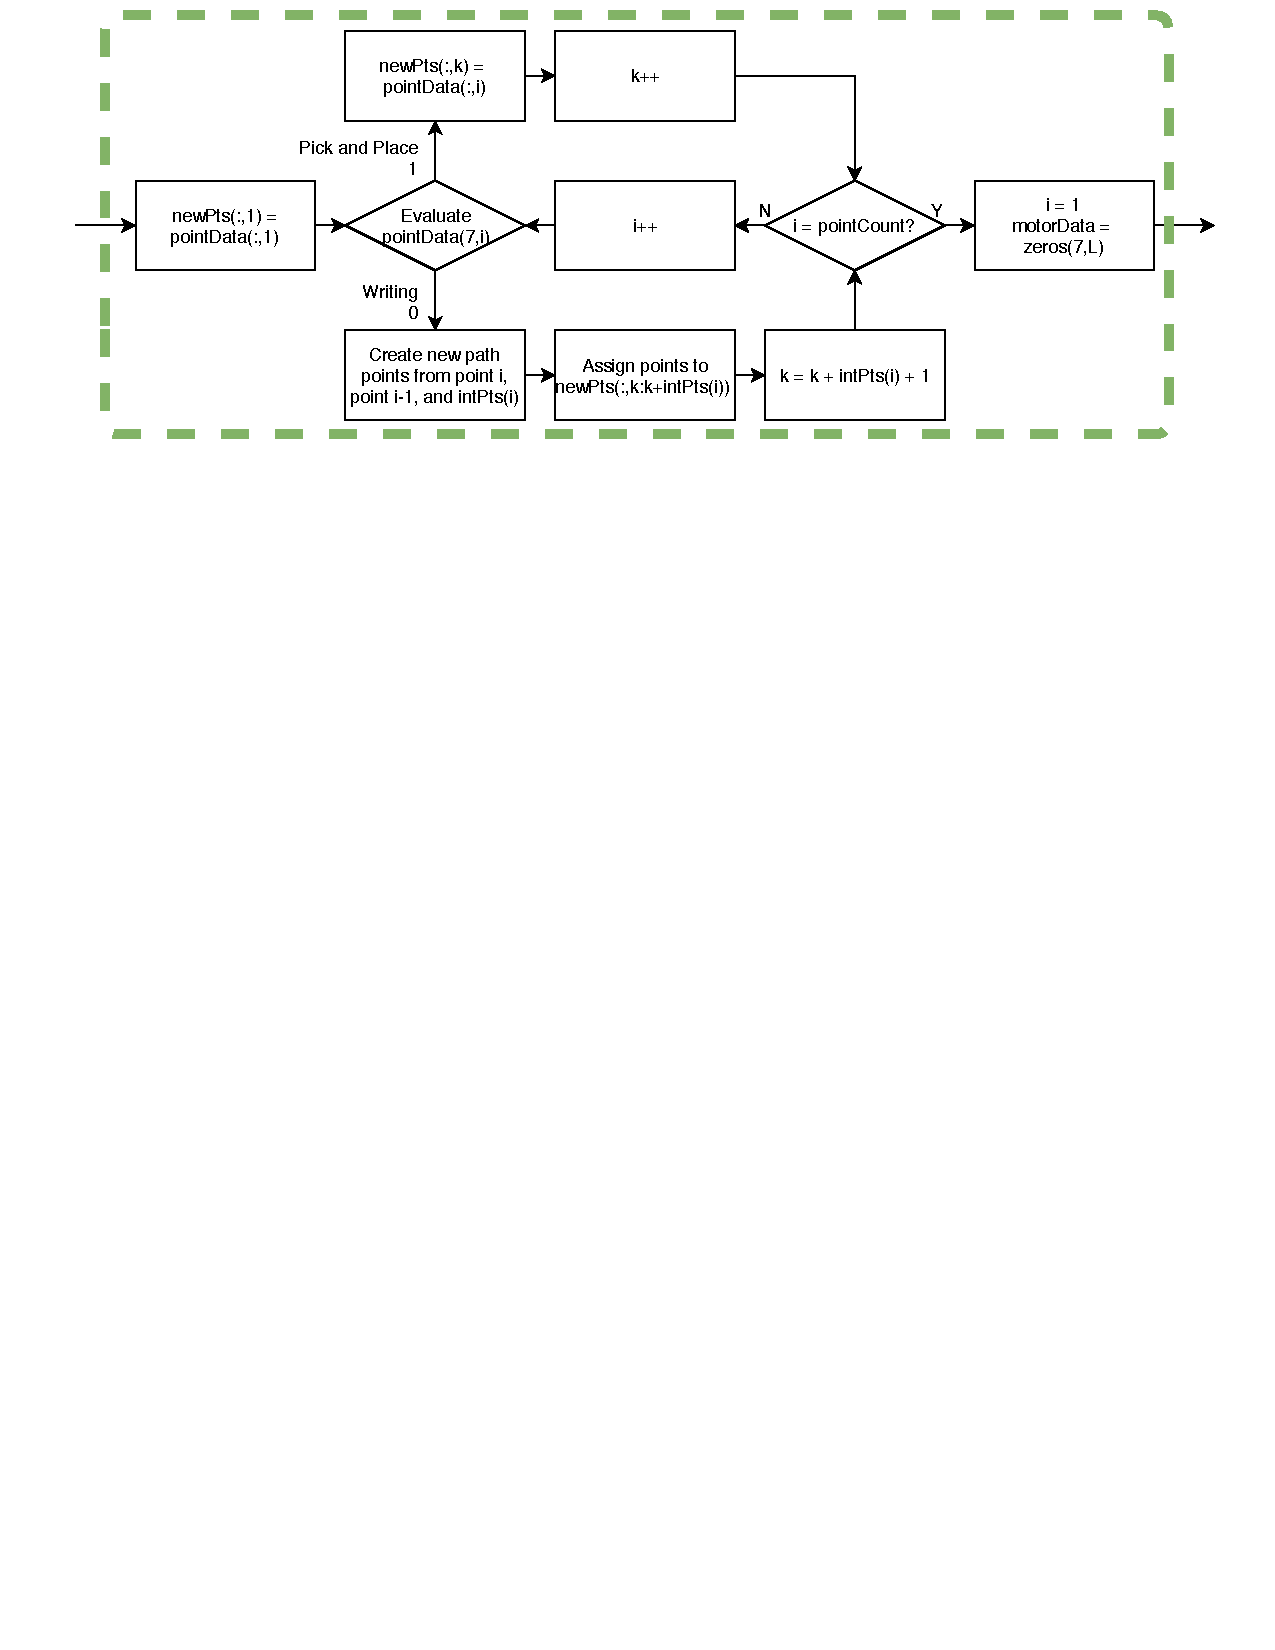
\includegraphics[width=.99\textwidth]{sf4}
  \caption{Software Flowchart Subsection 4}
  \label{fig:sf4}
  \end{subfigure}
\end{figure}
\looseness=-1

The code shown in \emph{Figure \ref{fig:sf4}} creates points every centimeter if the path type is cartesian straight line using the number of path points stored for each point from the previous block of software. This ensures that a straight line will be followed between the two user input points. If the path type is a straight line in the joint space, the software does not add any intermediate points since the path seen in the cartesian space does not matter.

The fifth code block in the flowchart calculates inverse kinematics of the points defined in the previous block of code and stores the angles as counts that can be used by the servos. The overview of this section can be seen in \emph{Figure \ref{fig:sf5}}.

\begin{figure}[htp] \ContinuedFloat
  \begin{subfigure}[c]{\textwidth}
  \center
  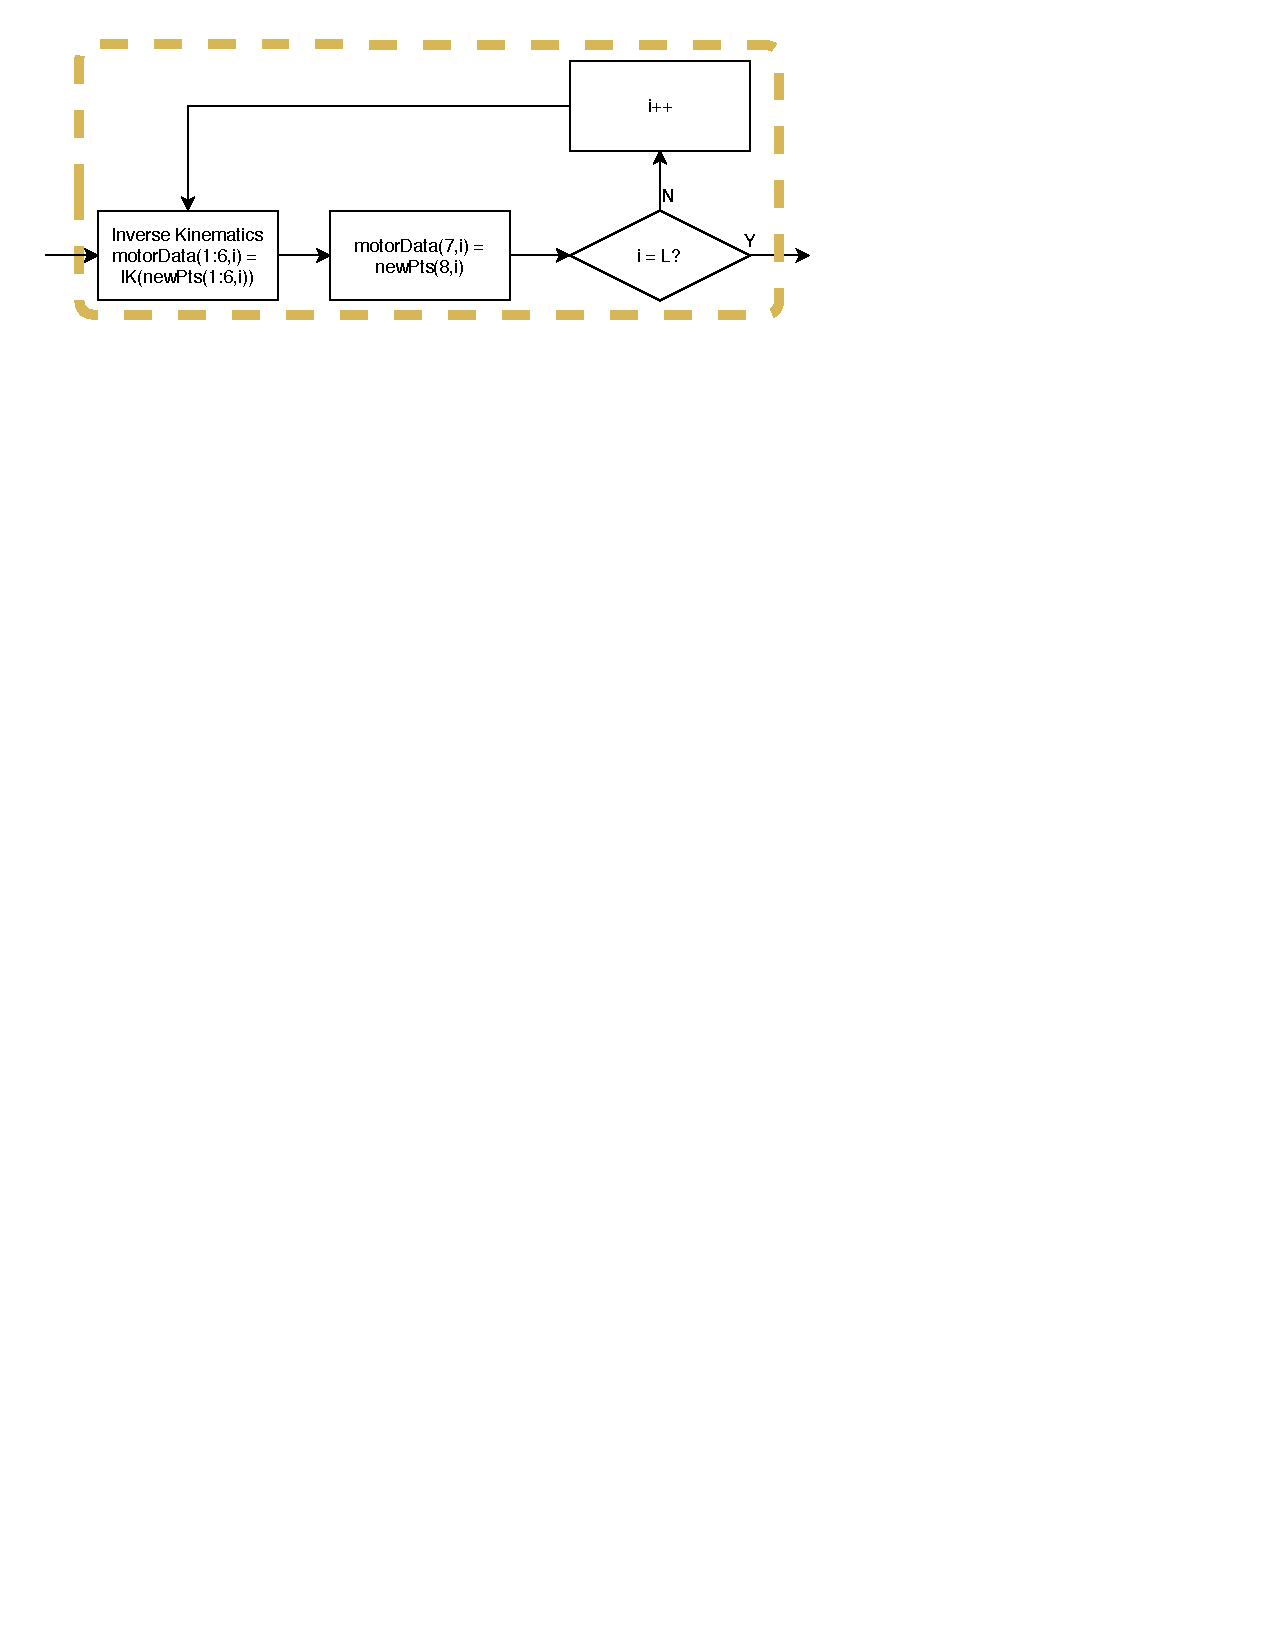
\includegraphics[width=\textwidth]{sf5}
  \caption{Software Flowchart Subsection 5}
  \label{fig:sf5}
  \end{subfigure}
\end{figure}

\emph{Figure \ref{fig:sf5}} shows that the new points found in the prior section of code are run through an inverse kinematics function that will output the necessary counts the servos can utilize. The code iterates through each point until the inverse kinematics have been calculated for all points.

The final block in the software diagram runs the manipulator through the desired task, with this section of code requiring user input at certain stages depending on the path type, seen in \emph{Figure \ref{fig:sf6}}.
\begin{figure}[htp] \ContinuedFloat
  \begin{subfigure}[c]{\textwidth}
  \center
  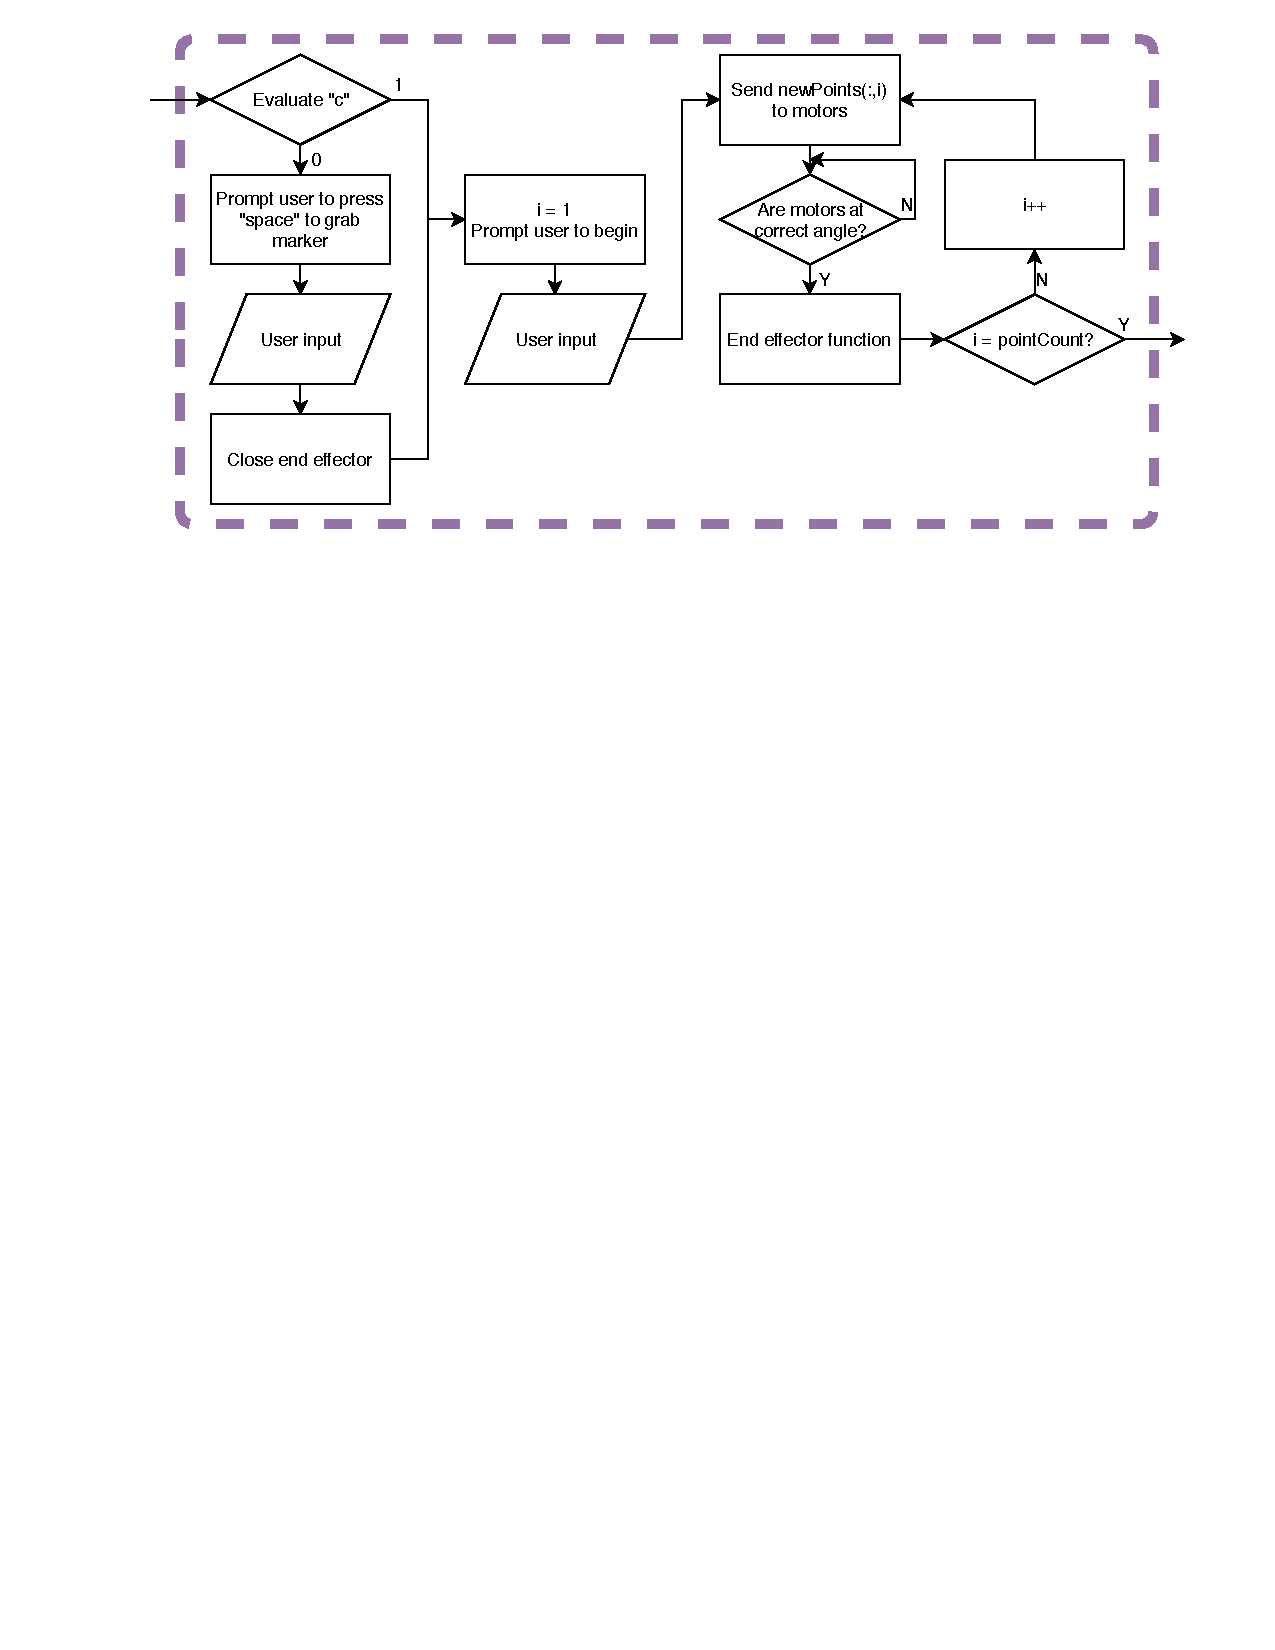
\includegraphics[width=\textwidth]{sf6}
  \caption{Software Flowchart Subsection 6}
  \label{fig:sf6}
  \end{subfigure}
\end{figure}

The code in \emph{Figure \ref{fig:sf6}} prompts the user to press space to close the end effector and grab the marker if drawing was the specified task, otherwise the software jumps straight into prompting the user to begin the task, and when the user begins the task the counts for each position are sent to the servos one at a time. The counts for the next position are not sent to the servos until the servos have reached the desired positions and the end effector function has been completed if there is one.
